\subsection{Chinese restaurant process}
Since $G \sim \DP(\alpha, H)$ is almost surely a discrete probability measure, if we draw $N$ observations $x_n \sim G$, we will only have $K \leq N$ unique observations $\{\bar x_k\}_{k = 1}^K$. We can view these as clusters. Let $\{z_n\}_{n = 1}^N$ be cluster indicators, i.e. $z_n = $ the cluster number of $x_n$ or equivalently $x_n = \bar x_{z_n}$. An equivalent version of \eqref{eqn:np/dp/polya/post-pred} can be written down, caring only about the cluster numbers:
\begin{equation}
	p(\tilde z \mid z_1, \dotsc, z_N, \alpha, H) = \frac{1}{\alpha + N} \left(\alpha \delta(\tilde z, K + 1) + \sum_{k = 1}^K N_k \delta(\tilde z, k)\right) \label{eqn:np/dp/crp/post-pred}
\end{equation}

We can get a sample from this distribution via the Chinese restaurant process, similar to the Pólya urn model in Algorithm~\ref{alg:np/dp/polya/polya}:
	\begin{algorithmbis}[Chinese restaurant process]\label{alg:np/dp/crp/crp}
        \begin{algorithmic}[1]
            \State Assume there are $K$ occupied tables (clusters) at the restaurant numbered from $1$ to $K$. The table $k$ has $N_k$ customers already sitting there (observations of cluster $k$), with the total of $N$ customers. A new customer sits at an occupied table $k$ with probability $\frac{N_k}{\alpha + N}$ and chooses a new table with probability $\frac{\alpha}{\alpha + N}$.
            \State New customer comes.
            \State The table number they choose follows the posterior predictive in \eqref{eqn:np/dp/crp/post-pred} (with $K + 1$ corresponding to choosing an unoccupied table).
        \end{algorithmic}
    \end{algorithmbis}

\begin{figure}[htp!]
	\centering
	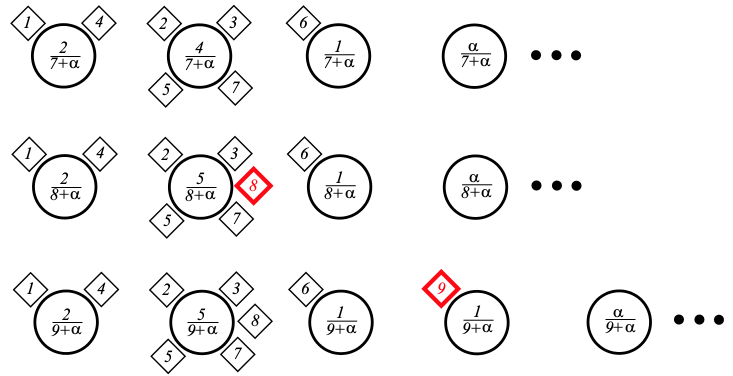
\includegraphics[width=1\textwidth]{np/dp/crp}
	\caption{(Figure from Suddherth PhD) Chinese restaurant process interpretation of the partitions induced by the Dirichlet process $\DP(\alpha, H)$. Tables (circles) are analogous to clusters, and customers (diamonds) to a series of observations. \emph{Top row}: A starting configuration, in which seven customers occupy three tables. Each table is labeled with the probability that the next customer sits there. \emph{Middle row}: New customers sit at occupied table $k$ with probability proportional to the number of previously seated diners $N_k$. In this example, the eighth customer joins the most popular, and hence likely, table. \emph{Bottom row}: Customers may also sit at one of the infinitely many unoccupied tables. The ninth diner does this.}
\end{figure}

The number of occupied tables $K$ almost surely approaches $\alpha \log(N)$ as $N \to \infty$.